\documentclass[landscape]{icsislides}

\usepackage[dvips]{graphicx}
%\usepackage[dvips]{color}
%\usepackage{subfigure}
\usepackage[T1]{fontenc}
\usepackage{psfrag}
\usepackage{xspace}
\usepackage{alltt}
\usepackage{colordvi}

\newcommand{\etc}{\emph{etc.}\xspace}
\newcommand{\ie}{\emph{i.e.,}\xspace}
\newcommand{\eg}{\emph{e.g.,}\xspace}

%\def\makeslidenum#1{\Gray{\fontseries{u}\selectfont#1}}%

%% XXX: comment-out to include logo
\newlogo{}

\begin{document}

%%======================================================================
\begin{titlepage}

\begin{center}
{\LARGE \Red{XORP: An eXtensible Open Router Platform}} \\
\vskip20pt

\vskip100pt
\begin{tabular}{c}
Atanu Ghosh \qquad Mark Handley \qquad Orion Hodson \\
Eddie Kohler \qquad \textbf{Pavlin Radoslavov} \\
\Gray{International Computer Science Institute}
\end{tabular}

\vskip-5pt
\begin{tabular}{c@{\qquad\qquad}c}
Adam Greenhalgh & Luigi Rizzo \\
\Gray{University College London} & \Gray{University of Pisa}
\end{tabular}
\end{center}

\end{titlepage}

% %%======================================================================
% \begin{titlepage}

% \begin{center}
% {\LARGE \bf XORP}
% \end{center}
% \vspace*{1.0in}
% \begin{center}
% Pavlin Radoslavov\\
% \vspace*{0.5in}
% \small {\it pavlin@icsi.berkeley.edu}\\
% \small International Computer Science Institute\\
% \small Berkeley, CA, USA
% \end{center}

% \end{titlepage}

%%======================================================================
\begin{slide}
\slidetitle{Outline}

\begin{enumerate}
  \item Motivations
  \item XORP introduction
  \item XORP IPC mechanism
  \item What does it take to implement a routing protocol?
  \item Dependency tracking mechanism
  \item Conclusions
\end{enumerate}

\end{slide}

%%======================================================================
\begin{slide}
\slidetitle{Networking research: divorced from reality?}

\begin{itemize}
  \item Gap between research and practice

  \item Most of the important Internet protocols originated in research

  \item It used to be that researchers designed systems, \emph{build
  implementations}, \emph{tried them out}, and standardized the ones that
  \emph{survived and proved useful}.

  \item What happened?

\end{itemize}

\end{slide}

%%======================================================================
\begin{slide}
\slidetitle{Networking research: why the divorce?}

\begin{itemize}
  \item The commercial Internet
  \begin{itemize}
    \item Network stability is critical, so experimentation is difficult
    \item Major infrastructure vendors not motivated to support
    experimentation
  \end{itemize}

  \item Network simulators
  \begin{itemize}
    \item Nice tool, but usually too abstract from reality
  \end{itemize}

\end{itemize}

\end{slide}

%%======================================================================
\begin{slide}
\slidetitle{Simulation is not a substitute for experimentation}

\begin{itemize}
  \item Many questions require real-world traffic and/or routing information

  \item Many people:
  \begin{itemize}
    \item Give up, implement their protocol in \emph{ns}
    \item Set \emph{ns} parameters based on guesses, existing scripts
    \item Write a paper that may or may not bear any relationship to reality
  \end{itemize}

  \item We need to be able to run experiments when required!

\end{itemize}

\end{slide}

%%======================================================================
\begin{slide}
\slidetitle{Options}

\begin{itemize}
  \item Option 1:
  \begin{itemize}
    \item Persuade Cisco to implement your protocol;
    \item Persuade ISPs that your protocol won't destabilize their networks;
    \item Conduct experiment.
  \end{itemize}

\end{itemize}

\end{slide}

%%======================================================================
\begin{slide}
\slidetitle{Options (cont.)}

\begin{itemize}
  \item Option 2:
  \begin{itemize}
    \item Implement routing protocol part in MRTd, GateD, or Zebra;
    \item Implement forwarding part in FreeBSD, Linux, Click, etc;
    \item Persuade network operators to replace their Ciscos with your PC;
    \item Conduct experiment.
  \end{itemize}

\end{itemize}

\end{slide}

%%======================================================================
\begin{slide}
\slidetitle{Likelihood of success?}

\begin{center}
  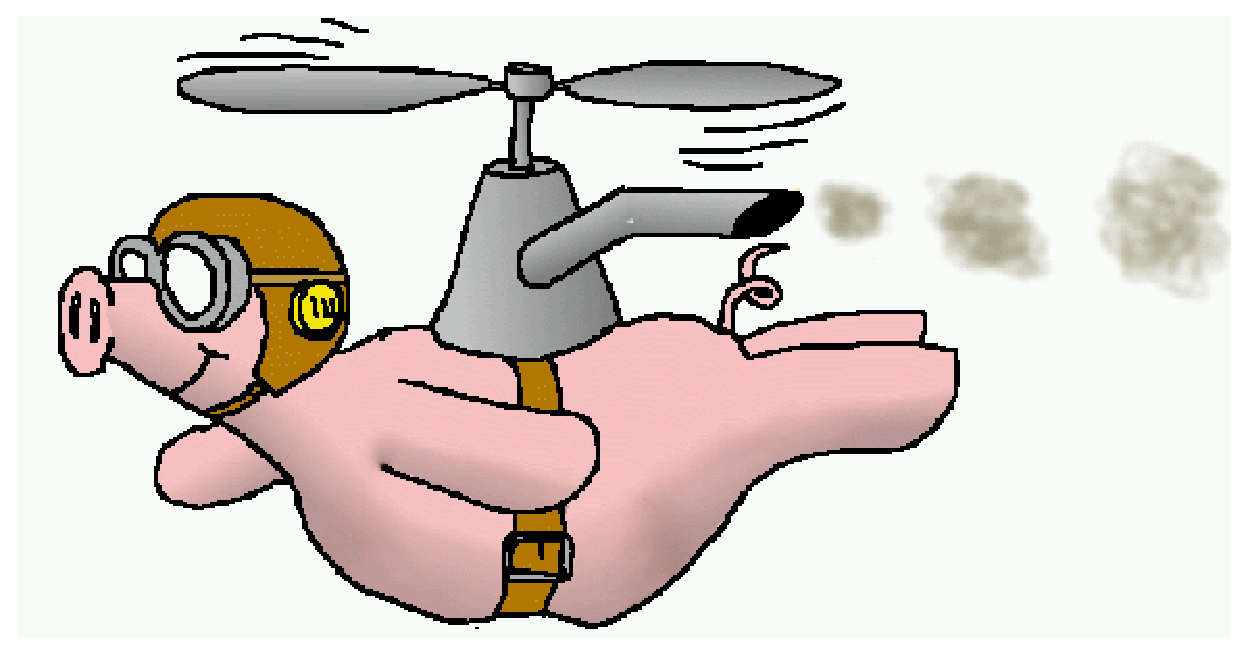
\includegraphics[width=6.0in]{figs/flyingpig}
\end{center}

\end{slide}

%%======================================================================
\begin{slide}
\slidetitle{Possible solutions}

\begin{itemize}

  \item Solution 1: A router vendor opens their development environment and
  APIs:
  \begin{itemize}
    \item Third-party router applications
    \item Basic router functionality cannot be changed
  \end{itemize}

  \item Solution 2: Someone (\emph{hint, hint}) builds a complete open-source
  router software stack explicitly designed for {\bf extensibility} and
  {\bf robustness}:
  \begin{itemize}
    \item Adventurous network operators deploy this router on their
    networks
    % it develops a reputation for stability and configurability.
    \item Result: a fully extensible platform suitable for {\bf research} and
    {\bf deployment}
  \end{itemize}
\end{itemize}

\end{slide}

%%======================================================================
\begin{slide}
\slidetitle{XORP: eXtensible Open Router Platform}

Complete software stack for an IP router:

\begin{itemize}
  \item Routing protocols: unicast and multicast
  \begin{itemize}
    \item Protocols can be run in simulation-like environment
  \end{itemize}
  \item Management Interfaces
  \item Forwarding path
\end{itemize}

\end{slide}

%%======================================================================
\begin{slide}
\slidetitle{XORP Architecture}

\begin{center}
  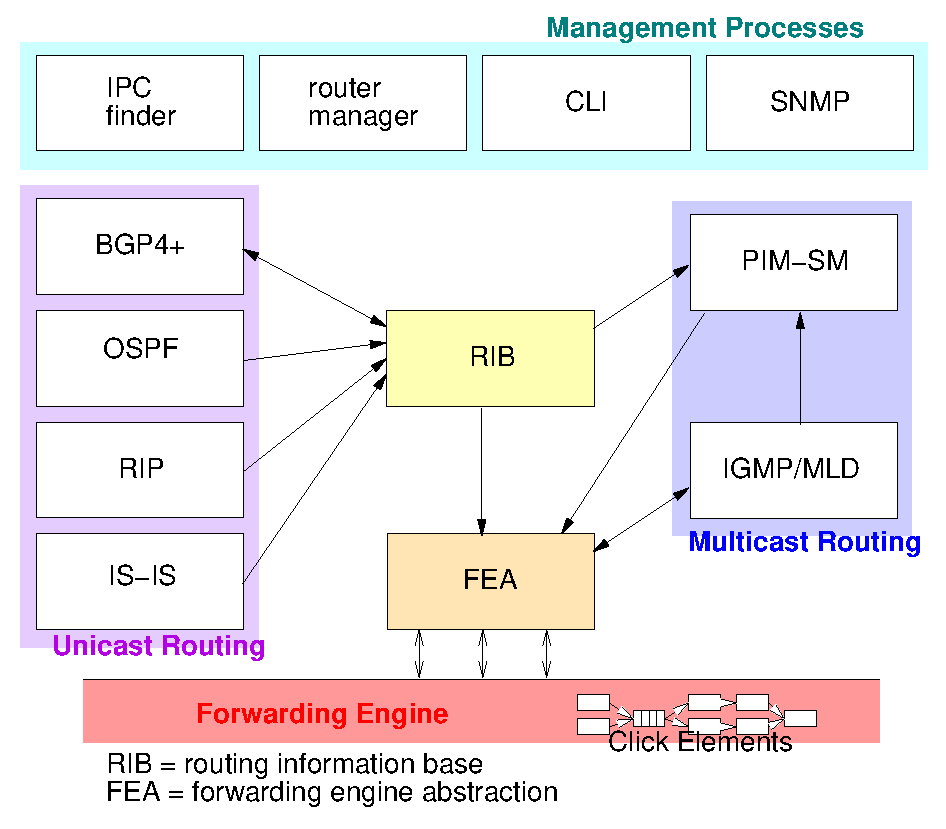
\includegraphics[width=6.0in]{figs/xorp_arch}
\end{center}

\end{slide}

%%======================================================================
\begin{slide}
\slidetitle{Challenges}

\begin{itemize}

  \item {\bf Features}: real-world routers support a long feature list

  \item {\bf Extensibility}:
  \begin{itemize}
    \item Every aspect of the router should be extensible
    \item Multiple extensions should be able to coexist
  \end{itemize}

  \item {\bf Performance}: raw forwarding performance; routing table size (not
  core routers; even edge routing is hard enough)

  \item {\bf Robustness}: must not crash or misroute packets

\end{itemize}

\end{slide}

%%======================================================================
\begin{slide}
\slidetitle{XORP Features}

\begin{itemize}

  \item IPv4 and \Gray{IPv6}

  \item Unicast routing protocols: BGP4+, OSPF, RIPv2/RIPng, \Gray{IS-IS}

  \item Multicast: PIM-SM/\Gray{SSM}, IGMPv1,2,\Gray{3}/MLDv1,\Gray{2}

  \item \Gray{DHCP, PPP}

  \item Management: CLI, \Gray{SNMP}, \Gray{WWW}

  \item Forwarding path: UNIX (native), Click

\end{itemize}

\end{slide}

%%======================================================================
\begin{slide}
\slidetitle{Extensibility: Intra-router APIs}

Separate abstract request (API) from concrete request (which process?
which arguments? which version?)

In particular, the caller:
\begin{itemize}
  \item Should not care about IPC mechanism
  \item Should not know in advance which process is relevant
  \dots unless required
\end{itemize}

\end{slide}

%%======================================================================
\begin{slide}
\slidetitle{Extensibility: XRLs (XORP Resource Locators)}

XORP IPC mechanism (like URLs for IPC):

\begin{center}
\texttt{finder://fea/fea/1.0/add\char`\_address4?vif:txt=fxp0\&addr:ipv4=10.0.0.1}
\vskip20pt
\end{center}

\begin{itemize}
  \item Library marshals arguments, implements transport, handles responses
  \item Redirection into a single XRL or an XRL sequence
  \item Programmer explicitly handles failure
\end{itemize}

\end{slide}

\def\LN#1{\setbox0\hbox{\lower\baselineskip\hbox{\rmfamily\BrickRed{#1}}}\wd0=0pt\ht0=0pt\dp0=0pt\box0\relax}
\def\RN#1{\setbox0\hbox{\lower\baselineskip\hbox to0pt{\hskip0pt plus-1000pt \rmfamily\BrickRed{#1}}}\ht0=0pt\dp0=0pt\box0\relax}
\let\t\texttt

%%======================================================================
\begin{slide}
\slidetitle{Extensibility: XRLs (XORP Resource Locators)}

XORP IPC mechanism (like URLs for IPC):

\begin{center}
\texttt{\LN{IPC mechanism: \t{finder}, \t{xudp}, \t{snmp}, \dots}\Red{finder}://fea/fea/1.0/add\char`\_address4?vif:txt=fxp0\&addr:ipv4=10.0.0.1}
\vskip20pt
\end{center}

\begin{itemize}
  \item Library marshals arguments, implements transport, handles responses
  \item Redirection into a single XRL or an XRL sequence
  \item Programmer explicitly handles failure
\end{itemize}

\end{slide}

%%======================================================================
\begin{slide}
\slidetitle{Extensibility: XRLs (XORP Resource Locators)}

XORP IPC mechanism (like URLs for IPC):

\begin{center}
\texttt{finder://\LN{Module/process name: \t{fea}, \t{rib}, \t{bgp}, \dots}\Red{fea}/fea/1.0/add\char`\_address4?vif:txt=fxp0\&addr:ipv4=10.0.0.1}
\vskip20pt
\end{center}

\begin{itemize}
  \item Library marshals arguments, implements transport, handles responses
  \item Redirection into a single XRL or an XRL sequence
  \item Programmer explicitly handles failure
\end{itemize}

\end{slide}

%%======================================================================
\begin{slide}
\slidetitle{Extensibility: XRLs (XORP Resource Locators)}

XORP IPC mechanism (like URLs for IPC):

\begin{center}
\texttt{finder://fea/\LN{Interface name: \t{fea}, \t{routing-process}, \dots}\Red{fea}/1.0/add\char`\_address4?vif:txt=fxp0\&addr:ipv4=10.0.0.1}
\vskip20pt
\end{center}

\begin{itemize}
  \item Library marshals arguments, implements transport, handles responses
  \item Redirection into a single XRL or an XRL sequence
  \item Programmer explicitly handles failure
\end{itemize}

\end{slide}

%%======================================================================
\begin{slide}
\slidetitle{Extensibility: XRLs (XORP Resource Locators)}

XORP IPC mechanism (like URLs for IPC):

\begin{center}
\texttt{finder://fea/fea/\LN{Version number}\Red{1.0}/add\char`\_address4?vif:txt=fxp0\&addr:ipv4=10.0.0.1}
\vskip20pt
\end{center}

\begin{itemize}
  \item Library marshals arguments, implements transport, handles responses
  \item Redirection into a single XRL or an XRL sequence
  \item Programmer explicitly handles failure
\end{itemize}

\end{slide}

%%======================================================================
\begin{slide}
\slidetitle{Extensibility: XRLs (XORP Resource Locators)}

XORP IPC mechanism (like URLs for IPC):

\begin{center}
\texttt{finder://fea/fea/1.0/\LN{Method name: \t{delete\char`\_address4},
\t{get\char`\_mtu}, \dots}\Red{add\char`\_address4}?vif:txt=fxp0\&addr:ipv4=10.0.0.1}
\vskip20pt
\end{center}

\begin{itemize}
  \item Library marshals arguments, implements transport, handles responses
  \item Redirection into a single XRL or an XRL sequence
  \item Programmer explicitly handles failure
\end{itemize}

\end{slide}

%%======================================================================
\begin{slide}
\slidetitle{Extensibility: XRLs (XORP Resource Locators)}

XORP IPC mechanism (like URLs for IPC):

\begin{center}
\texttt{finder://fea/fea/1.0/add\char`\_address4?\LN{Arguments}\Red{vif:txt=fxp0\&addr:ipv4=10.0.0.1}}
\vskip20pt
\end{center}

\begin{itemize}
  \item Library marshals arguments, implements transport, handles responses
  \item Redirection into a single XRL or an XRL sequence
  \item Programmer explicitly handles failure
\end{itemize}

\end{slide}

%%======================================================================
\begin{slide}
\slidetitle{Defining XRL interface}

XRL interface is defined in XRL-specific files:

\begin{verbatim}
interface pim/0.1 {
	/**
	 * Enable a PIM virtual interface.
	 *
	 * @param vif_name the name of the vif to enable.
	 * @param fail true if failure has occurred.
	 * @param reason contains failure reason if it occurred.
	 */
	enable_vif	? vif_name:txt	-> fail:bool & reason:txt

	...
}
\end{verbatim}

\end{slide}

%%======================================================================
\begin{slide}
\slidetitle{Using XRLs: C++}

All header files are auto-generated; developer implements only XRL handlers:

\begin{verbatim}
XrlCmdError XrlPimNode::pim_0_1_enable_vif(
    // Input values, 
    const string&       vif_name, 
    // Output values, 
    bool&               fail,
    string&             reason)
{
    fail = enable_vif(vif_name, reason);
    return XrlCmdError::OKAY();
}
\end{verbatim}

\end{slide}

%%======================================================================
\begin{slide}
\slidetitle{Using XRLs: Shell Script}

Everything is ASCII text:

\begin{verbatim}
pim_enable_vif()
{
    vif_name=$1
    XRL="finder://$PIM_TARGET/pim/0.1/enable_vif"
    XRL_ARGS="?vif_name:txt=$vif_name"
    call_xrl $XRL$XRL_ARGS
}
\end{verbatim}

\end{slide}

%%======================================================================
\begin{slide}
\slidetitle{Extensibility: RIB}

\begin{center}
  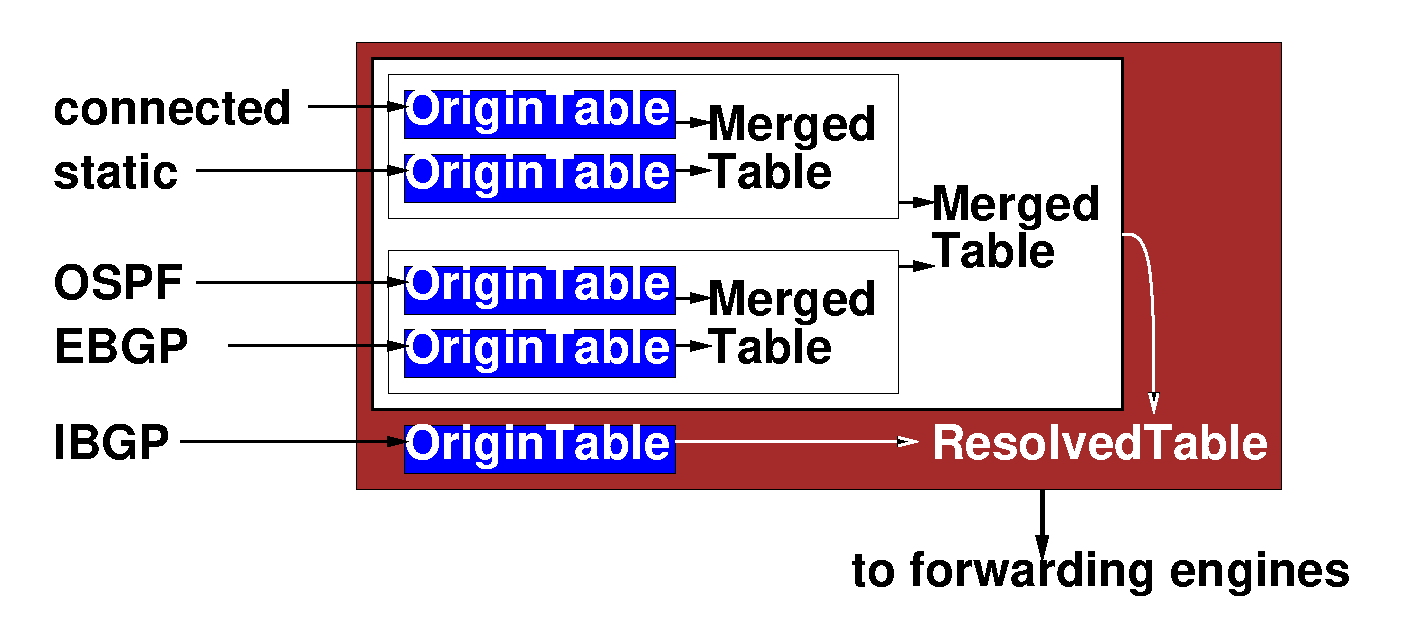
\includegraphics[width=8.0in]{figs/routingtable}
\end{center}

\begin{itemize}
  \item Object-oriented routing table design
  \item Add new merged tables implementing new merging policies, \dots
\end{itemize}

\end{slide}

%%======================================================================
\begin{slide}
\slidetitle{Extensibility/performance: Click forwarding path}

\begin{center}
  \includegraphics[width=2.5in]{figs/ipr.1}
\end{center}

Fast kernel forwarding; easy to write extensions

\end{slide}

%%======================================================================
\begin{slide}
\slidetitle{Robustness}

\begin{itemize}

  \item Policy decision: Strong robustness for user-level processes
  \begin{itemize}
    \item Difficult to get performance, robustness, and extensibility
    simultaneously
  \end{itemize}

  \item Facilitated by multi-process design
  \begin{itemize}
    \item Automatically restart processes that crash
  \end{itemize}

  \item XRL sandboxes
  \begin{itemize}
    \item All interaction with router through XRLs
    \item Redirect XRLs to run new protocols in a sandbox
  \end{itemize}

\end{itemize}

\end{slide}

%%======================================================================
\begin{slide}
\slidetitle{Improving robustness and performance: distributed router}

\begin{itemize}

  \item XRLs can be sent across network

  \item Each routing process can run on a separate machine

  \item Only the FEA must run on the machine with the forwarding engine:
  \begin{itemize}
    \item The memory and the CPU are not the bottleneck
    \item Improved robustness through hot-swapping of routing modules
  \end{itemize}

\end{itemize}

\end{slide}

%%======================================================================
\begin{slide}
\slidetitle{Example of a distributed router}

\begin{center}
  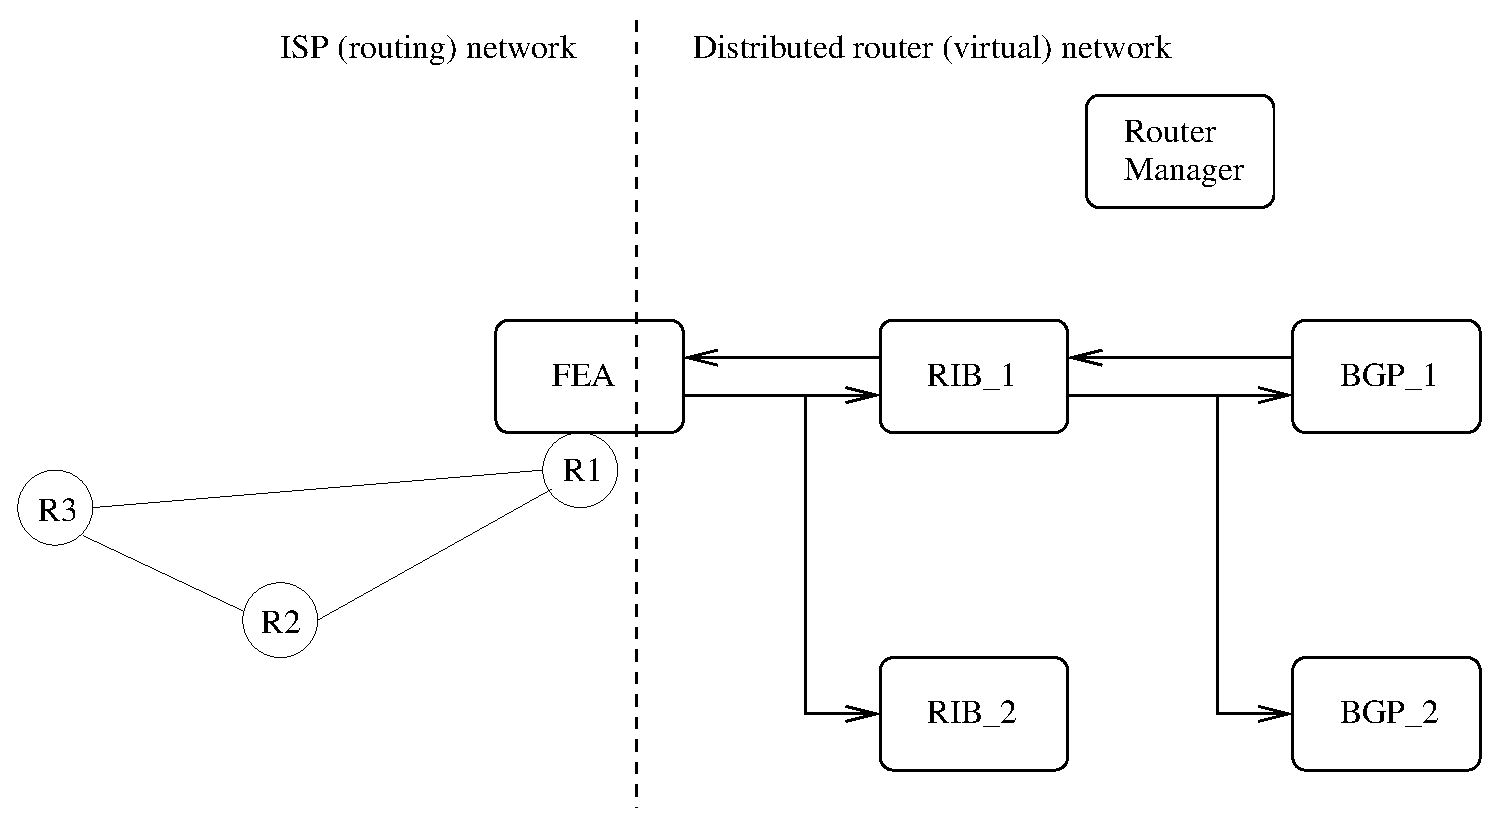
\includegraphics[width=8.0in]{figs/distributed_router}
\end{center}

\end{slide}

%%======================================================================
\begin{slide}
\slidetitle{Distributed router (cont.)}

\begin{itemize}

  \item The Router Manager coordinates the modules and the interaction among
  them.

  \item A routing protocol instance doesn't care whether it is part of a
  distributed router, or whether it is running as a backup

  \item Potential issues:
  \begin{itemize}
  \item Communication latency
  \item Bandwidth overhead
  \item Synchronization
  \end{itemize}

\end{itemize}

\end{slide}

%%======================================================================
\begin{slide}
\slidetitle{What does it take to implement a routing protocol?}

PIM-SM (Protocol Independent Multicast-Sparse Mode): case-study

\begin{itemize}

  \item Fairly complicated protocol (protocol specification is 100 + 25
  pages), full of tiny details:
  \begin{itemize}
    \item Early specifications (two RFCs) easy to read, difficult to decode and
    implement
    \item Lastest spec is much more ``implementor-friendly''
  \end{itemize}

  \item Lots of routing state and state dependency

\end{itemize}

\end{slide}

%%======================================================================
\begin{slide}
\slidetitle{0. Get yourself into the right mindset}

Think \Red{SIMPLICITY} and \Red{CONSISTENCY}:

\begin{itemize}

  \item Simplicity gives you lots of space for maneuvers

  \item Consistency (\eg in variables naming): things don't get into your way
  when you shuffle them around

  \item Which one comes first would be a trade-off

  \item Don't go into extremes

\end{itemize}

\end{slide}

%%======================================================================
\begin{slide}
\slidetitle{Forget (for now) the word ``optimization''!!}

PIM-SM may have lots of routing state:

\begin{itemize}
  \item So what, by the time the implementation is ready for prime-time, the
  price of memory will fall in half!

  \item Premature optimization results in complicated design, which is a sure
  sign for disaster!

  \item Solve performance issues when you do testing and profiling (\ie after
  the implementation is completed)

\end{itemize}

\end{slide}

%%======================================================================
\begin{slide}
\slidetitle{1. Design and understand the interaction with other modules}

\begin{center}
  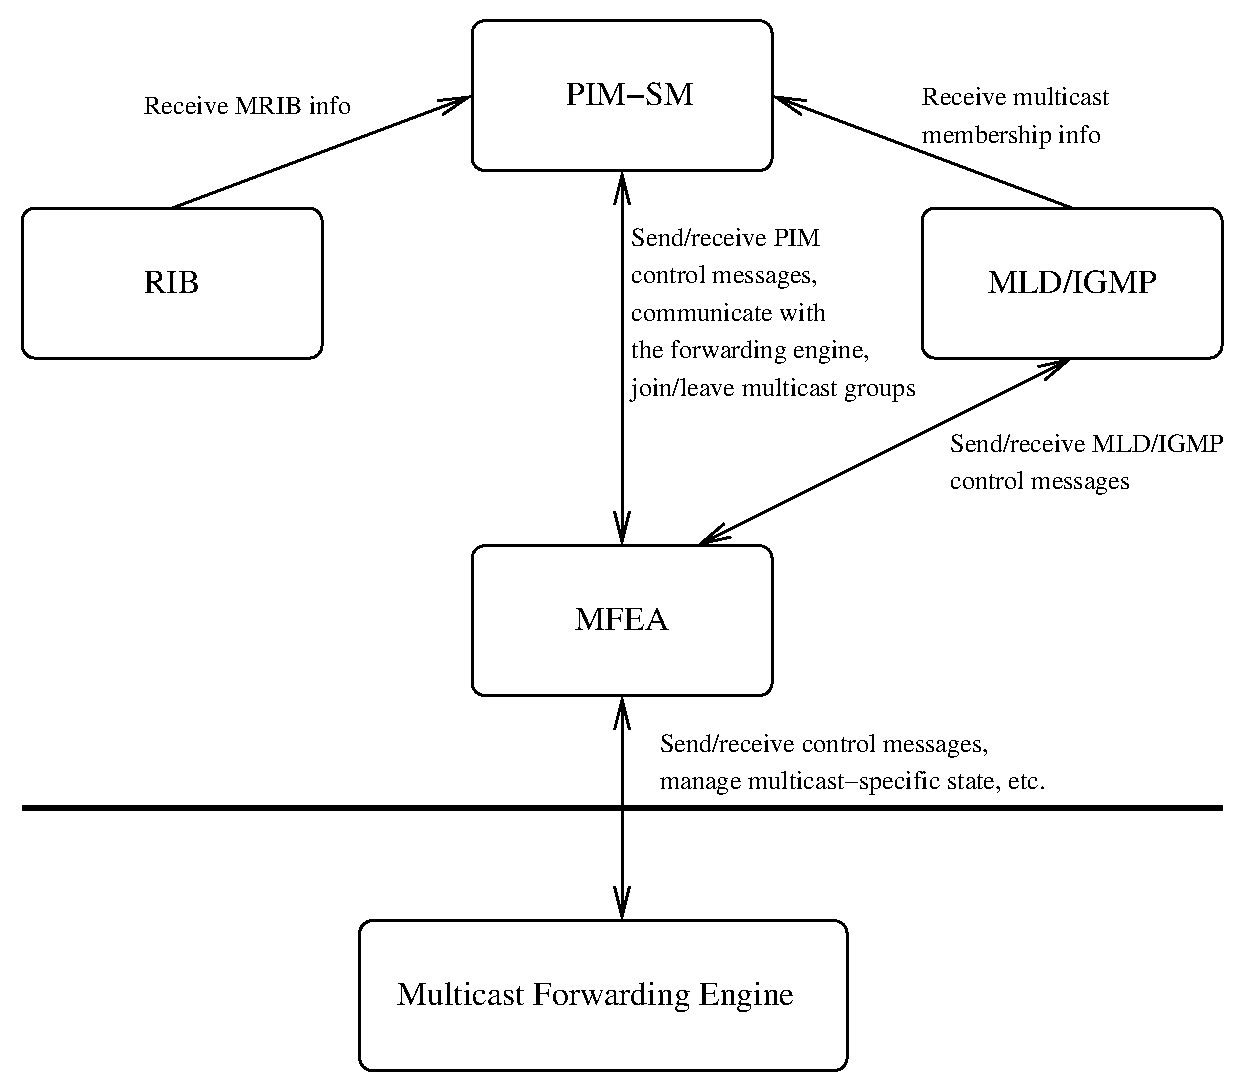
\includegraphics[width=6.0in]{figs/pim_other_modules_interaction}
\end{center}

% For now don't worry about the details.

\end{slide}

%%======================================================================
\begin{slide}
\slidetitle{2. Break-down the protocol into semi-independent units}

\begin{center}
  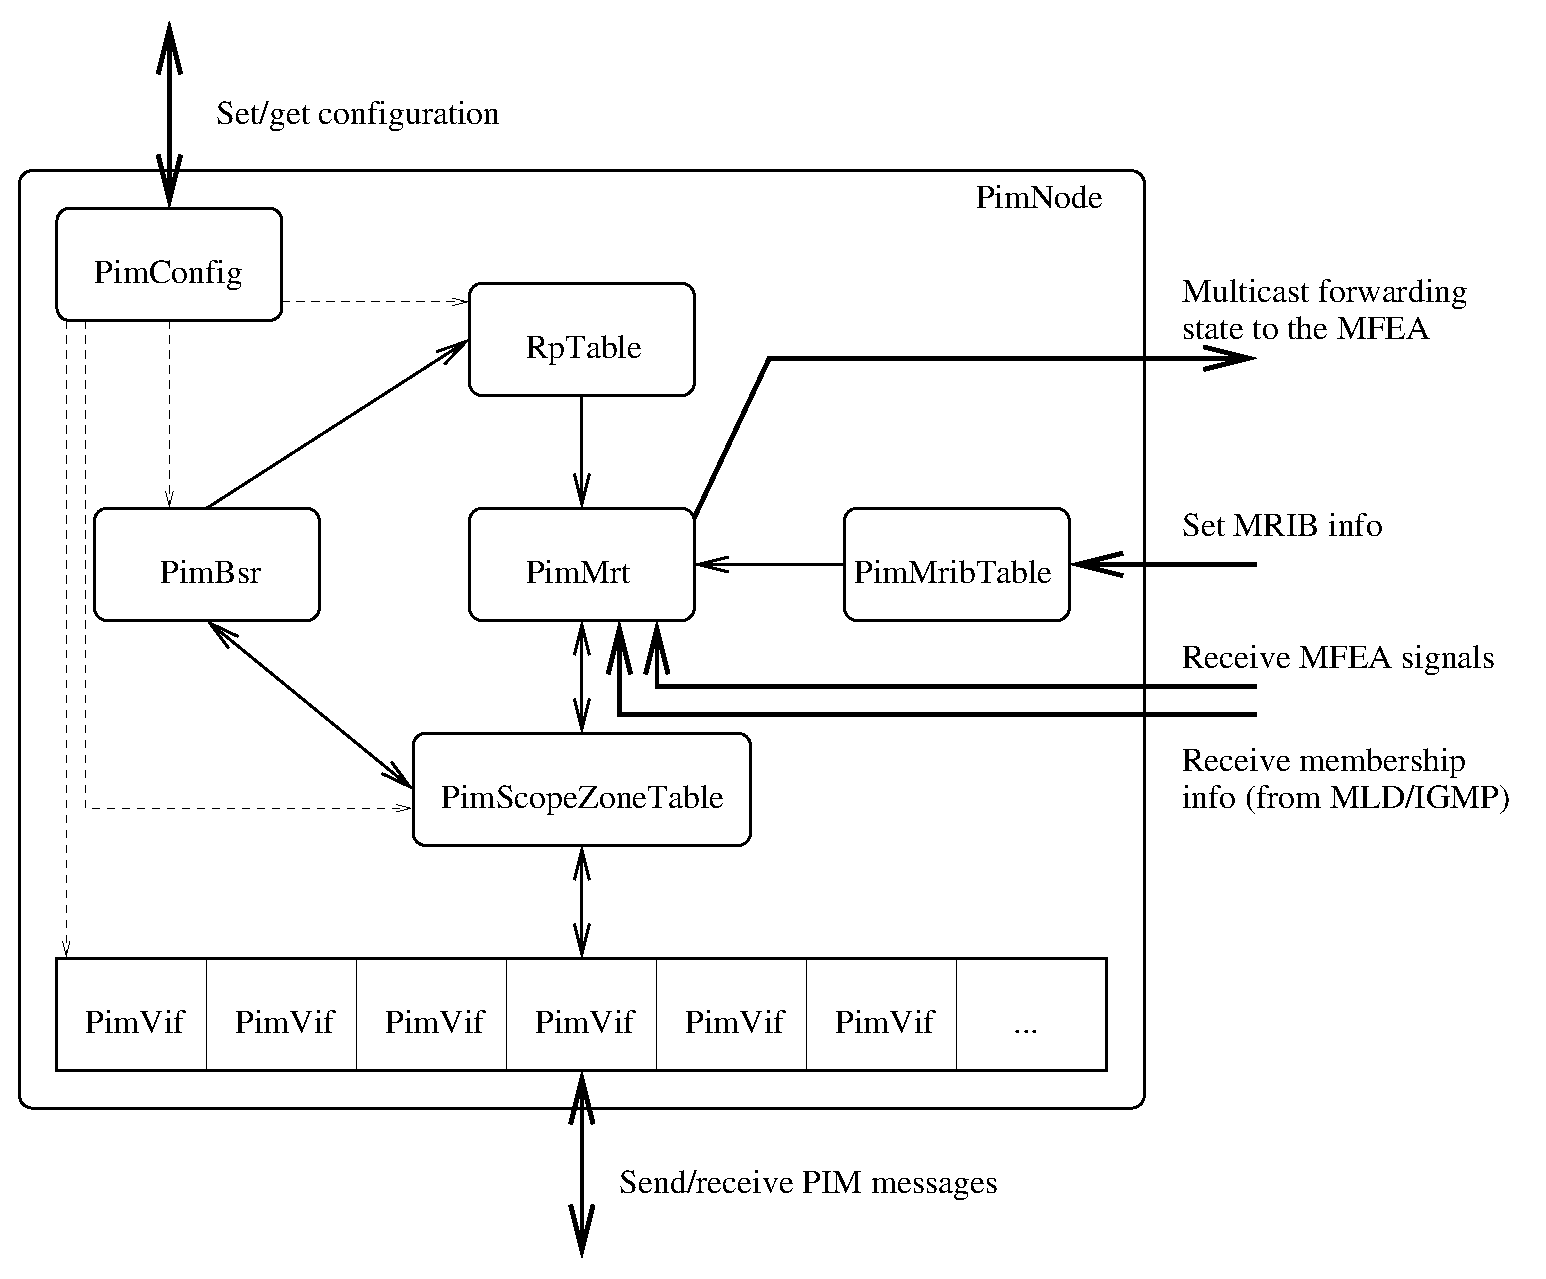
\includegraphics[width=6.0in]{figs/pim_design_overview}
\end{center}

\end{slide}

%%======================================================================
\begin{slide}
\slidetitle{Protocol units break-down}

\begin{itemize}

  \item Probably the most difficult part

  \item There is no way you will get it right the first time!

  \item Simplicity comes first!

\end{itemize}

\end{slide}

%%======================================================================
\begin{slide}
\slidetitle{3. Protocol units implementation}

\begin{itemize}

  \item If you got your design right, in this stage you need to concentrate
  only on the protocol detail

  \item Be consistent!

  \item Each unit must respond to common methods/commands. E.g.:
  start/stop/enable/disable.

  \item Try to avoid implementation-specific assumptions

\end{itemize}

\end{slide}

%%======================================================================
\begin{slide}
\slidetitle{4. Testing, testing, testing}

\begin{itemize}

  \item If you don't test it, it doesn't work!

  \item Detailed testing takes time

  \item If you can, build a testing framework that allows you to perform
  automated testing any time you change something

  \item Now you can profile and optimize

\end{itemize}

\end{slide}

%%======================================================================
\begin{slide}
\slidetitle{Dependency tracking mechanism}

\begin{itemize}

  \item For each input event, what are the operations to perform and their
  ordering

  \item If the protocol is simple, you can take care of this by hand

  \item Unfortunately, this is not the case with PIM-SM:
  total of 50 input events, and 70 output operations.   

\end{itemize}

\end{slide}

%%======================================================================
\begin{slide}
\slidetitle{PIM-SM dependency tracking mechanism}

PIM-SM spec has tens of macros like:

\begin{small}
\begin{verbatim}
pim_include(S,G) =
    { all interfaces I such that:
      ( (I_am_DR( I ) AND lost_assert(S,G,I) == FALSE )
        OR AssertWinner(S,G,I) == me )
       AND  local_receiver_include(S,G,I) }
\end{verbatim}
\end{small}

The corresponding state dependency rule is:
\begin{small}
\begin{verbatim}
void
PimMreTrackState::track_state_pim_include_sg(list<PimMreAction> action_list)
{
    track_state_i_am_dr(action_list);
    track_state_lost_assert_sg(action_list);
    track_state_assert_winner_sg(action_list);
    track_state_local_receiver_include_sg(action_list);
}
\end{verbatim}
\end{small}

\end{slide}

%%======================================================================
\begin{slide}
\slidetitle{Dependency tracking}

\begin{center}
  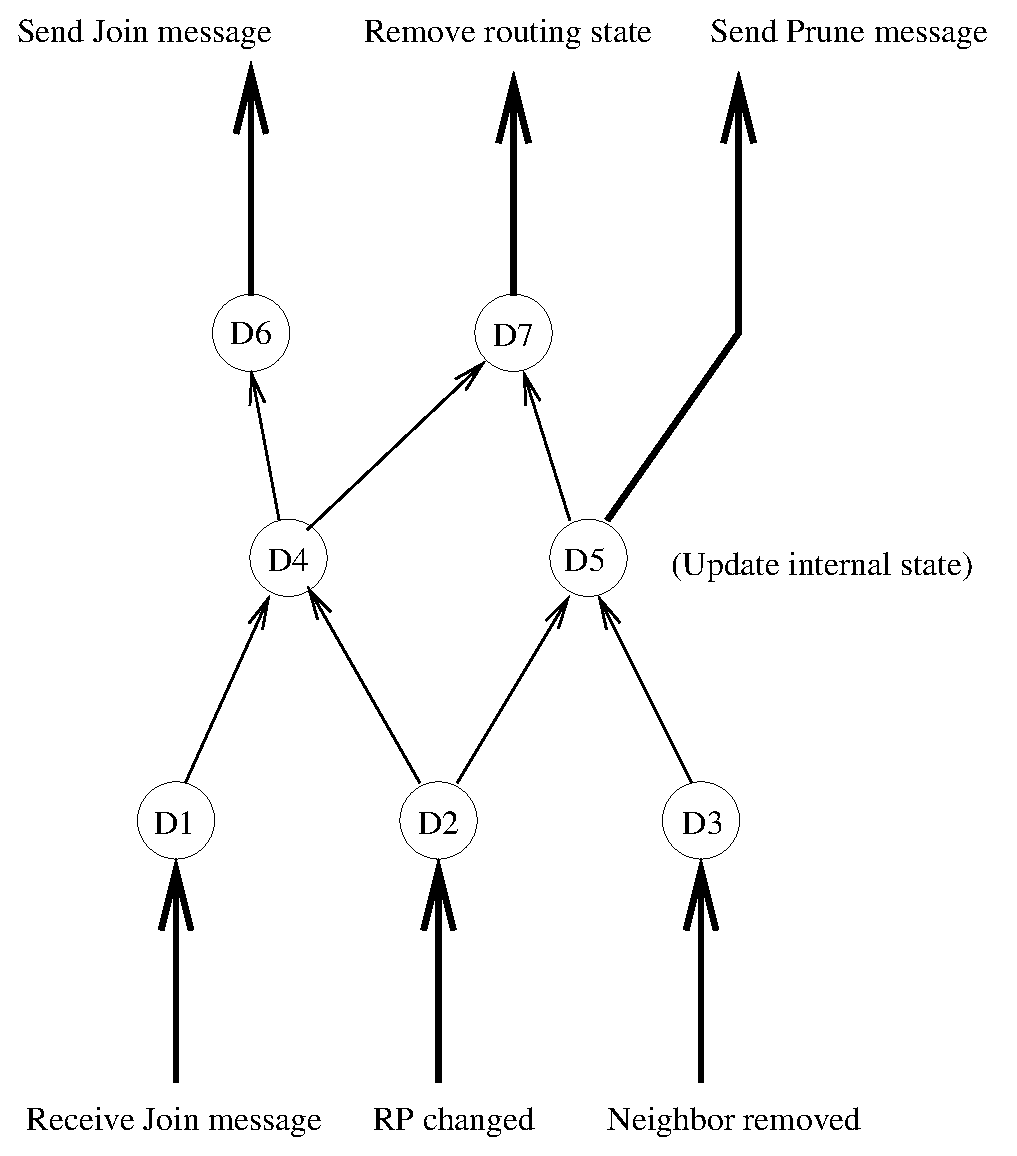
\includegraphics[scale=0.6]{figs/pim_state_dependency}
\end{center}

\end{slide}

%%======================================================================
\begin{slide}
\slidetitle{Dependency tracking (2)}

\begin{center}
  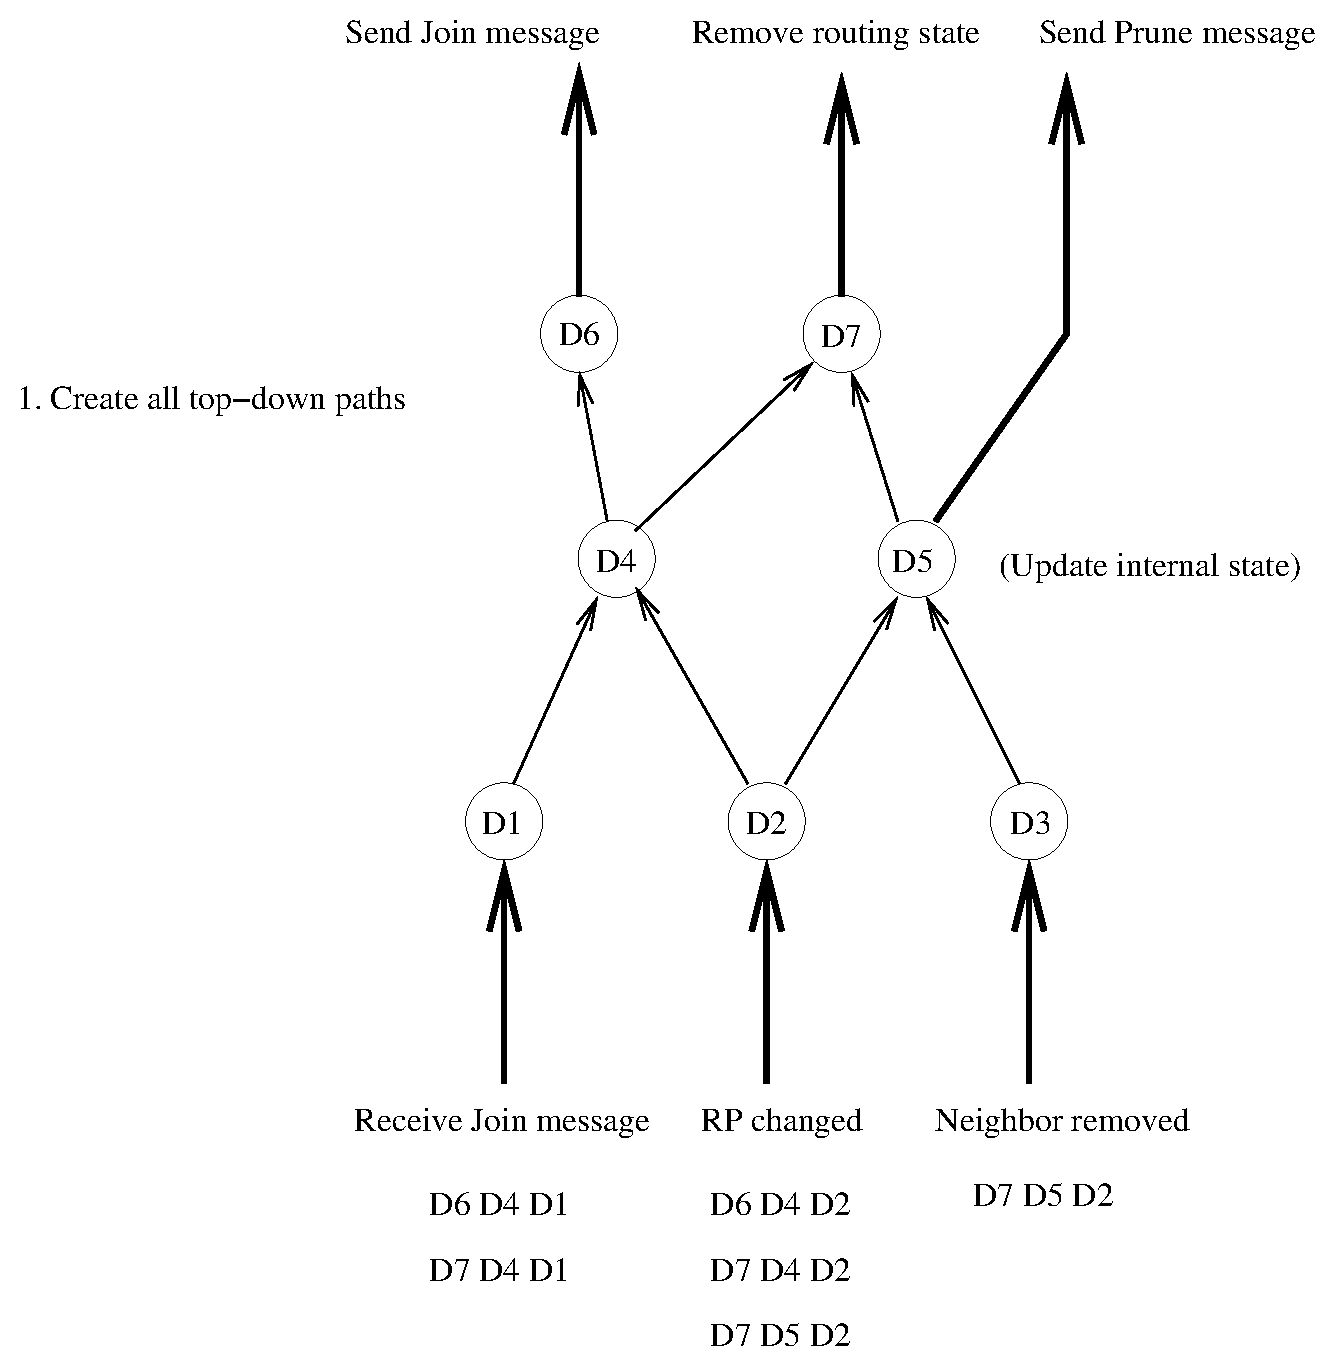
\includegraphics[scale=0.6]{figs/pim_state_dependency2}
\end{center}

\end{slide}

%%======================================================================
\begin{slide}
\slidetitle{Dependency tracking (3)}

\begin{center}
  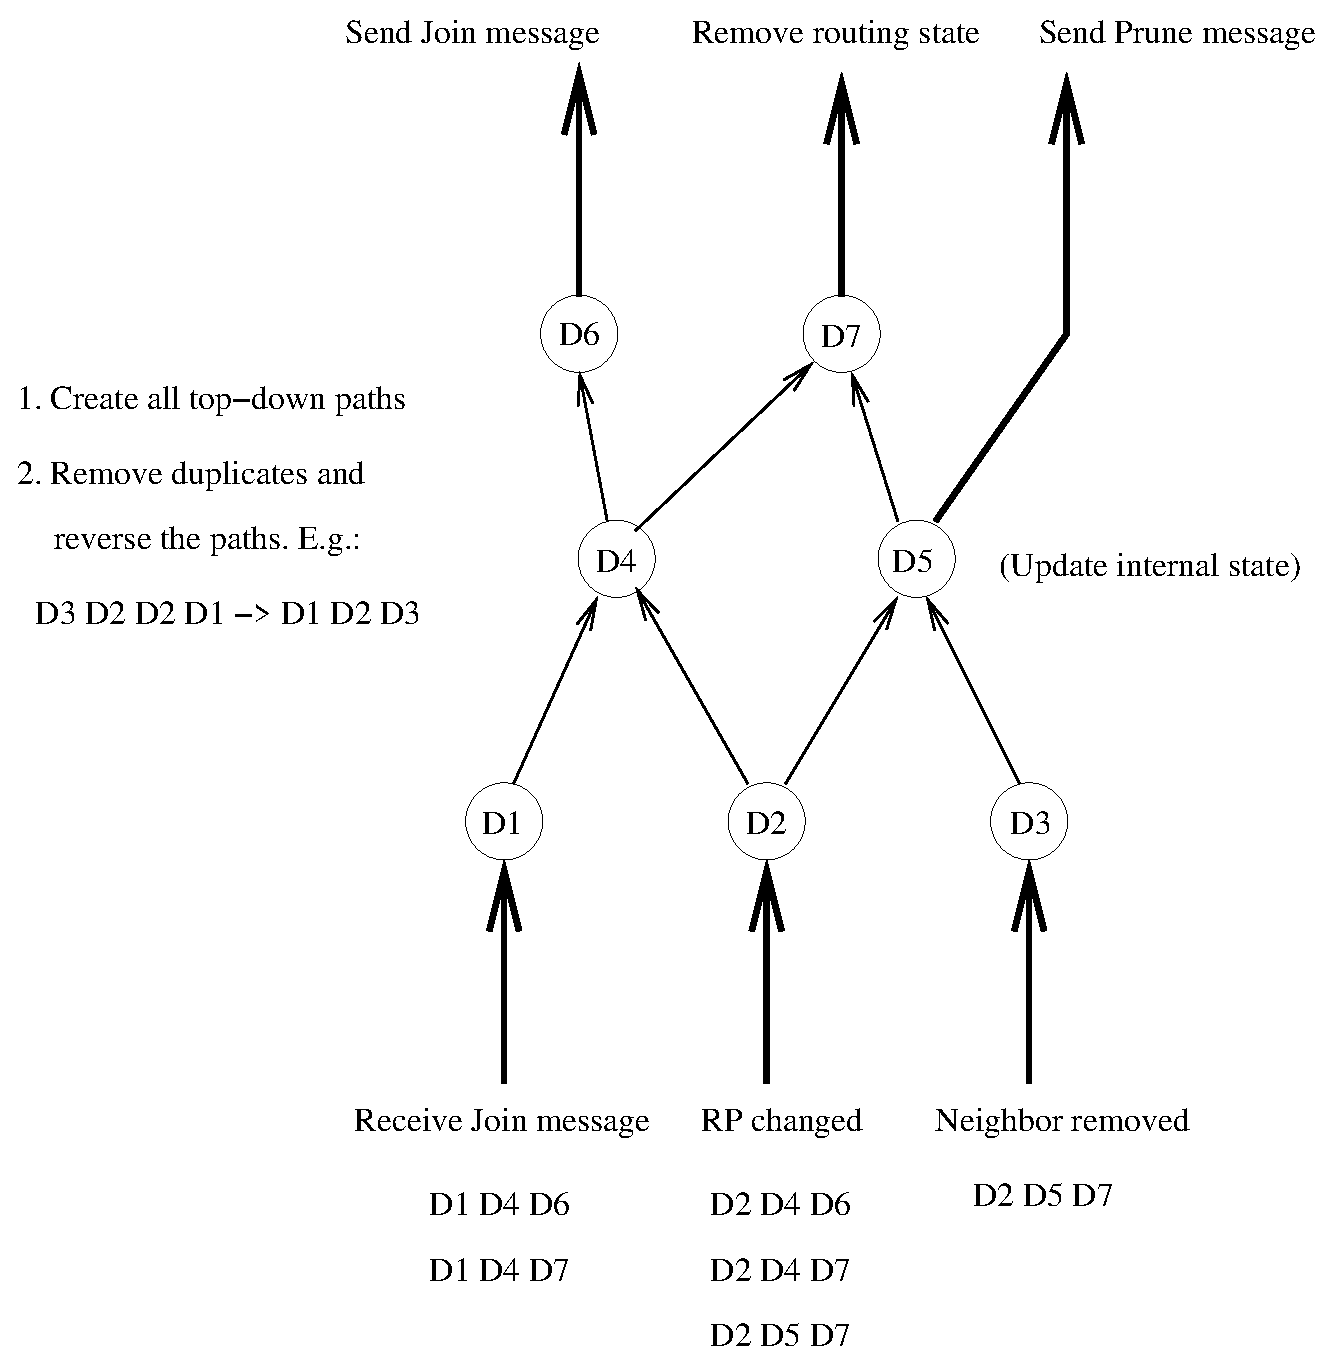
\includegraphics[scale=0.6]{figs/pim_state_dependency3}
\end{center}

\end{slide}

%%======================================================================
\begin{slide}
\slidetitle{Dependency tracking (4)}

\begin{center}
  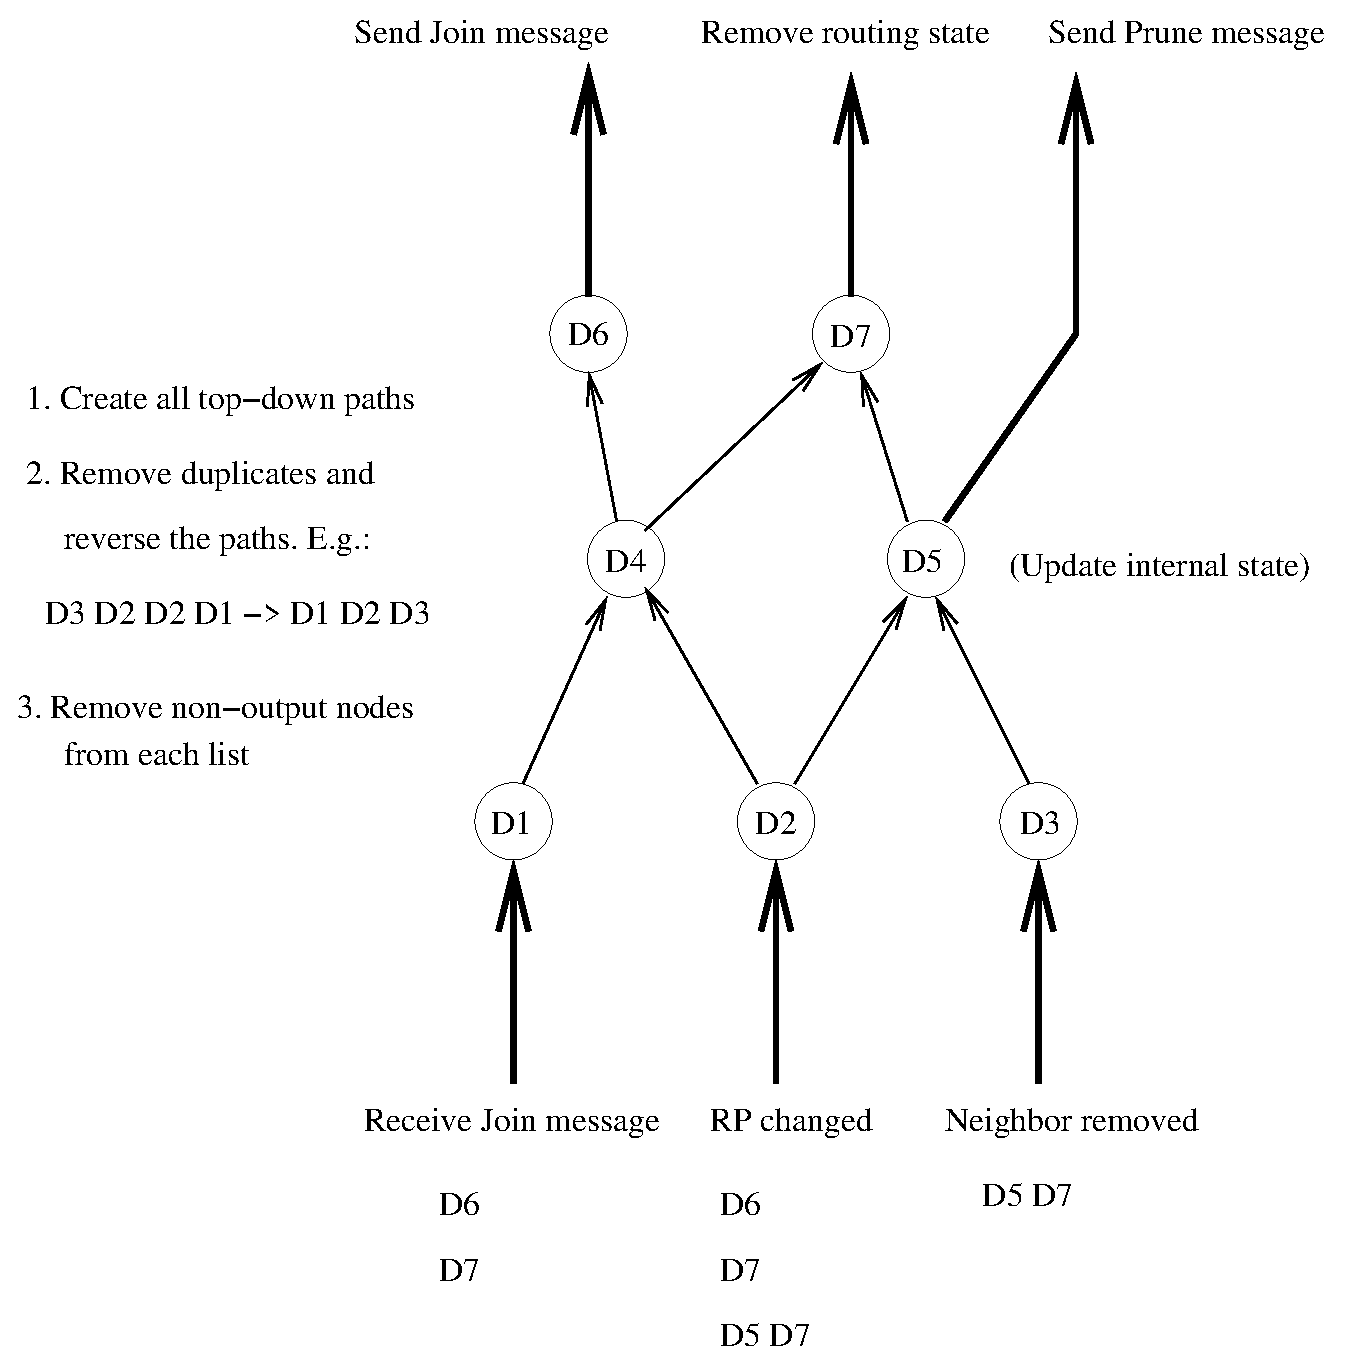
\includegraphics[scale=0.6]{figs/pim_state_dependency4}
\end{center}

\end{slide}

%%======================================================================
\begin{slide}
\slidetitle{Dependency tracking (5)}

\begin{center}
  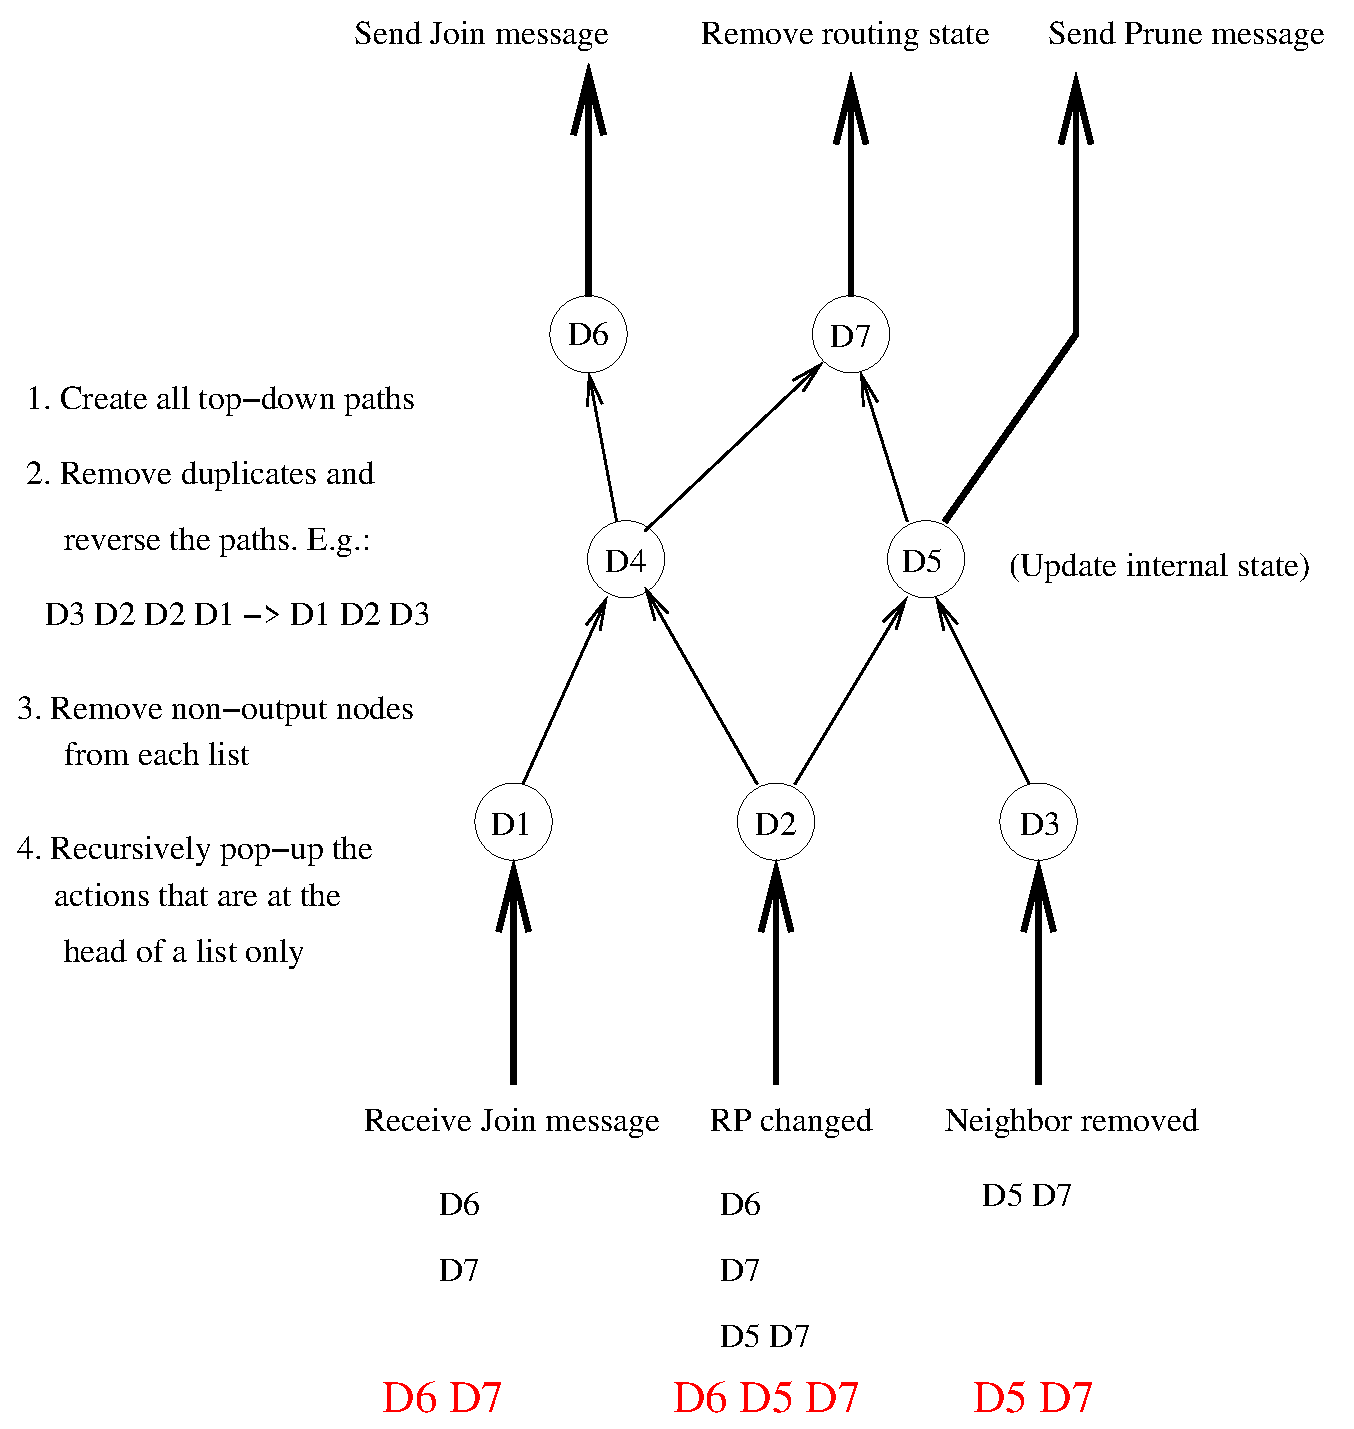
\includegraphics[scale=0.6]{figs/pim_state_dependency5}
\end{center}

\end{slide}

%%======================================================================
\begin{slide}
\slidetitle{Dependency tracking usage}

\begin{itemize}
  \item The unidirectional ``graph'' is semi-defined by the state computation
  macros

  \item For each macro, write the corresponding state dependency rule

  \item All state dependency is pre-computed once on start-up

  \item If the spec changes, the rules are easy to update

  \item If the spec does not use macros for state computation, write your own
  macros

\end{itemize}

\end{slide}

%%======================================================================
\begin{slide}
\slidetitle{Status}

\begin{itemize}

  \item Completed: core design, IPC, RIB, BGP, PIM-SM, IGMP, FEA

  \item In progress: OSPF, RIP adaptation, IPv6, Click integration,

  \item Future work: create XORP simulation environment

  \item First preliminary release early December: \\
  {\bf http://www.xorp.org/}

\end{itemize}

\end{slide}

%%======================================================================
\begin{slide}
\slidetitle{Summary}

\begin{itemize}

  \item XORP tries to close the gap between {\bf research} and {\bf practice}

  \item Routing architecture designed for {\bf extensibility} and {\bf
  robustness}.

  \item Can be used to build distributed routers

  \item XORP simulation environment can facilitate protocol development: the
  simulation and the real-world prototype use exactly same code

\end{itemize}

\end{slide}

%%======================================================================
\end{document}
